\documentclass[t,xcolor={svgnames}]{beamer}

\mode<presentation>
\usetheme{Warsaw}
\useoutertheme{infolines} 

\usepackage{fontspec}
\usepackage{lmodern}
\usepackage{amsmath}
\usepackage{amsfonts}
\usepackage{bbm}
\usepackage{bm}
\usepackage[font=small,labelfont=bf]{caption} % Required for specifying captions to tables and figures
\usepackage{nicefrac}
\usepackage{color}
\usepackage{perpage}
\usepackage{multirow}
\usepackage{multicol}
\usepackage{adjustbox}
\usepackage{tikz}
\usepackage{tikz-dependency}
\usepackage{tikz-qtree}
\usepackage{tikz,pgfplots,pgfplotstable}
\usetikzlibrary{arrows.meta,graphs,graphs.standard,graphdrawing,quotes,shapes}
\usegdlibrary{layered,trees}

\tikzset{
  invisible/.style={opacity=0},
  visible on/.style={alt={#1{}{invisible}}},
  alt/.code args={<#1>#2#3}{%
    \alt<#1>{\pgfkeysalso{#2}}{\pgfkeysalso{#3}} % \pgfkeysalso doesn't change the path
  },
}

\captionsetup{labelformat=empty}
\newcommand{\parser}[1]{TUPA\textsubscript{#1}}

\newfontfamily\hebfont[Script=Hebrew, Scale=MatchUppercase]{FreeSans}
\newcommand{\heb}[1]{\bgroup\textdir TRT\hebfont #1\egroup}

\makeatletter
\pgfdeclareshape{vector}{
      \inheritsavedanchors[from={rectangle}]
      \inheritbackgroundpath[from={rectangle}]
      \inheritanchorborder[from={rectangle}]
      \foreach \x in {center,north east,north west,north,south,south east,south west,east,west}{
        \inheritanchor[from={rectangle}]{\x}
      }

    \backgroundpath{
      \pgftransformshift{\pgfpoint{-16pt}{-4pt}}
          \draw[rounded corners=2pt] (0,0) rectangle (32pt,8pt);
    }

    \beforebackgroundpath{
      \draw[step=8pt,help lines,-] (8pt,.1pt) grid (24pt,7.9pt);
    }
}
\pgfdeclareshape{vector}{
      \inheritsavedanchors[from={rectangle}]
      \inheritbackgroundpath[from={rectangle}]
      \inheritanchorborder[from={rectangle}]
      \foreach \x in {center,north east,north west,north,south,south east,south west,east,west}{
        \inheritanchor[from={rectangle}]{\x}
      }

    \backgroundpath{
      \pgftransformshift{\pgfpoint{-16pt}{-4pt}}
          \draw[rounded corners=2pt] (0,0) rectangle (32pt,8pt);
    }

    \beforebackgroundpath{
      \draw[step=8pt,help lines,-] (8pt,.1pt) grid (24pt,7.9pt);
    }
}
\makeatother

\MakePerPage{footnote}

% Outline slides
\AtBeginSection
{\begin{frame} \frametitle{Outline} \tableofcontents[currentsection,currentsubsection] \end{frame}}
\AtBeginSubsection
{\begin{frame} \frametitle{Outline} \tableofcontents[currentsection,currentsubsection] \end{frame}}


\begin{document}


\title[]{Universal Semantic Parsing with Neural Networks}
\author{Daniel Hershcovich}
\institute[]{PhD Lecture}
\date{February 5, 2019}

\begin{frame}
\titlepage
\end{frame}

\begin{frame}
\frametitle{Natural Language Processing: What's It Good For?}
\onslide<1>{Machine translation:}
\begin{center}
\onslide<1,4>{
  \fbox{After graduation, John moved to Copenhagen}

  $\downarrow$
}

\only<1,3>{
  \fbox{\heb{אחרי שג'ון סיים את הלימודים, הוא עבר לקופנהגן}}
}
\only<2,4>{
  \fbox{\heb{אחרי ש\underline{\heb{ג'ון}} סיים את הלימודים, הוא עבר ל\underline{\heb{קופנהגן}}}}
}
\end{center}

\vspace{-7mm}
  
\only<2>{
  \vspace{-5mm}

  Named entity \\
  recognition:

  \hspace{28mm} $\downarrow$ \hspace{48mm} $\downarrow$

  \hspace{22.9mm} Location \hspace{36.7mm} Person
}

\only<3>{
  Text \\
  simplification:
  
  \vspace{-1cm}
}
  
\only<3,4>{  
  \begin{center}
  $\downarrow$
  
  \fbox{\heb{ג'ון סיים את הלימודים. ג'ון עבר לקופנהגן.}}
  \end{center}
}

\only<4>{
  Sequence-to-sequence sometimes works, but lacks inductive bias.

  \begin{center}
    \begin{tikzpicture}[->]
    \tikzstyle{main}=[circle, minimum size=7mm, draw=black!80, node distance=12mm]
    \foreach \i in {1,3,7,9} {
        \node[main, fill=white!100] (h\i) at (\i,0) {};
        \node[main, fill=white!100] (o\i) at (\i.5,2) {};
    }
    \node (h5) at (5.5,0) {$\ldots$};
    \node (o5) at (5.5,2) {$\ldots$};
    \foreach \current/\next in {1/3,3/5,5/7,7/9} {
        \path (h\current) edge (h\next);
        \path (o\current) edge (o\next);
    }
    \foreach \i in {1,3,7,9} {
      \foreach \j in {1,3,7,9} {
        \path[gray!50] (h\i) edge (o\j);
      }
    }
    \end{tikzpicture}
  \end{center}
}

\end{frame}

\begin{frame}
\frametitle{Linguistic Structure Annotation Schemes}
Represent structure as a graph.

\vfill

Example: {\color{DarkBlue}syntactic}/{\color{DarkRed}semantic} bi-lexical dependencies

\vfill

    \begin{adjustbox}{center}
    \begin{dependency}[line width=1.5pt]
        \begin{deptext}[column sep=2.5em,ampersand replacement=\^,font=\rmfamily]
    	You \^ want \^ to \^ take \^ a \^ long \^ bath \\
        \end{deptext}
        \deproot[draw=DarkBlue]{2}{root}
        \depedge[draw=DarkBlue]{2}{1}{nsubj}
        \depedge[edge start x offset=-4pt,draw=DarkBlue]{2}{4}{xcomp}
        \depedge[draw=DarkBlue]{2}{3}{mark}
        \depedge[draw=DarkBlue]{4}{7}{dobj}
        \depedge[draw=DarkBlue]{7}{5}{det}
        \depedge[draw=DarkBlue]{7}{6}{amod}
        \deproot[edge below,edge style={DarkRed},edge unit distance=1em]{2}{top}
        \depedge[edge below,draw=DarkRed]{2}{4}{ARG2}
        \depedge[edge below,draw=DarkRed]{2}{1}{ARG1}
        \depedge[edge below,draw=DarkRed,edge unit distance=1.6em,edge start x offset=6pt]{4}{1}{ARG1}
        \depedge[edge below,draw=DarkRed]{4}{7}{ARG2}
        \depedge[edge below,draw=DarkRed]{5}{7}{BV}
        \depedge[edge below,draw=DarkRed]{6}{7}{ARG1}
    \end{dependency}
    \end{adjustbox}
\end{frame}

\begin{frame}
    \frametitle{Semantic Representations}
Semantic representation schemes
abstract away from syntactic detail that does not affect meaning:
\begin{center}
    \fbox{\textrm{bathed}} = \fbox{\textrm{took a bath}}
    
    \vspace{1cm}
    
    \fbox{\textrm{graduated}} = \fbox{\heb{סיים את הלימודים}}
\end{center}
\end{frame}


\def\semanticrepresentations{
\begin{frame}
    \frametitle{Semantic Representations}

      \begin{flushright}
        \scalebox{.6}{
\begin{tikzpicture}[level distance=2cm, sibling distance=25mm, ->, draw=Indigo]
    \node[font=\bf\sffamily\small,Indigo] at (-3,0) {UCCA:};
    \node (ROOT) [fill=Indigo, circle] {}
      child {node (After) {After} edge from parent node[left] {\scriptsize $L$\;}}
      child {node (graduation) [fill=Indigo, circle] {}
      {
        child {node {graduation} edge from parent node[left] {\scriptsize $P$}}
      } edge from parent node[left] {\scriptsize $H$} }
      child {node {,} edge from parent node[right] {\scriptsize $U$}}
      child {node (moved) [fill=Indigo, circle] {}
      {
        child {node (John) {John} edge from parent node[left] {\scriptsize $A$}}
        child {node {moved} edge from parent node[left] {\scriptsize $P$}}
        child {node [fill=Indigo, circle] {}
        {
          child {node {to} edge from parent node[left] {\scriptsize $R$}}
          child {node {Copenhagen} edge from parent node[left] {\scriptsize $C$}}
        } edge from parent node[left] {\scriptsize $A$} }
      } edge from parent node[right] {\scriptsize $H$} }
      ;
    \draw[dashed,->] (graduation) to node [auto] {\scriptsize $A$} (John);
\end{tikzpicture}
        }
      \end{flushright}
    
    \vspace{-23mm}
    
    \scalebox{.6}{
\begin{tikzpicture}
\node[font=\bf\sffamily\small,DarkGreen] at (0,6) {AMR:};
\graph[layered layout, sibling distance=4cm, layer distance=2cm, nodes={ellipse,draw=DarkGreen}, edges={nodes={sloped}, DarkGreen}]{
a4 Copenhagen[as={Copenhagen}];
a2 John[as={John}];
a1[as={person}];
a0[as={move-01}];
a3[as={city}];
a2[as={name}];
a5[as={after}];
a4[as={name}];
a6[as={graduate-01}];

a1 ->  ["name"' above] a2;
a0 ->  ["ARG0"' above] a1;
a0 ->  ["ARG2"' above] a3;
a0 ->  ["time"' above] a5;
a3 ->  ["name"' above] a4;
a2 ->  ["op1"' above] a2 John;
a5 ->  ["op1"' above] a6;
a4 ->  ["op1"' above] a4 Copenhagen;
};
\draw[->, above, DarkGreen] (a6) to node[sloped] {ARG0} (a1);
\end{tikzpicture}
      }
    \vspace{-15mm}
    
    \begin{flushright}
    \begin{minipage}{.01\textwidth}
    {\color{DarkRed}\bf\sffamily\tiny SDP:}
    \end{minipage}
    \begin{minipage}{.6\textwidth}
        \rmfamily
        \scalebox{.7}{
\begin{dependency}[theme=simple,edge style={-{Latex[length=2mm]}, color=DarkRed},
            text only label, label style={above, color=DarkRed, font=\bf\ttfamily}, font=\small]
    \begin{deptext}[column sep=1em,ampersand replacement=\^]
	After \^ graduation \^ , \^ John \^ moved \^ to \^ Copenhagen \\
    \end{deptext}
    \deproot{5}{top}
    \depedge{1}{2}{ARG2}
    \depedge{1}{5}{ARG1}
    \depedge{5}{4}{ARG1}
    \depedge{6}{5}{ARG1}
    \depedge{6}{7}{ARG2}
\end{dependency}
    }
    \end{minipage}
    \end{flushright}
\end{frame}}

\semanticrepresentations


\section{Background: The UCCA Semantic Representation Scheme}

\begin{frame}
\frametitle{Universal Conceptual Cognitive Annotation (UCCA)}
Cross-linguistically applicable \cite{abend2013universal}. \\
Stable in translation \cite{sulem2015conceptual}. \\
Rapid and intuitive annotation by non-experts.

\vfill

\begin{adjustbox}{center}
            \begin{tikzpicture}[level distance=8mm, sibling distance=5mm,
                draw=Indigo,
                every node/.append style={font=\rmfamily},
            	every circle node/.append style={fill=Indigo}]
                \begin{scope}[frontier/.style={distance from root=25mm}]
                \Tree [.\node [circle] (root u) {};
                  \edge node [auto=right]{L}; \node (After u) {After};
                  \edge node[auto=right]{H};
                  [.\node [circle](an appleu) {};
                    \edge node[auto=right]{P}; \node (graduation u) {graduation};
                  ]
                  \edge node[auto=right]{};
                  [.\node [circle](John moved to Paris u) {};
                    \edge node[auto=right]{A}; \node (John u) {John};
                    \edge node[auto=left]{P}; \node (moved u) {moved};
                    [.\node [circle](John moved to Paris u) {};
                      \edge node[auto=right]{R}; \node (to u) {to};
                      \edge node[auto=left]{C}; \node (Paris u) {Paris};
                    ]
                  ]
                ]
                \end{scope}
                \begin{scope}[yshift=-41mm,grow'=up, frontier/.style={distance from root=12mm}]
                \Tree [.\node [circle] (rootd) {};
                  \edge node [auto=left]{}; \node (After d) {\heb{אחרי}};
                  \edge node[auto=right]{}; \node (gave) {gave};
                  \edge node[auto=right]{};\node (John) {John};
                  \edge node[auto=right]{};
                  [.\node [circle] (an appled) {};
                    \edge node[auto=left]{}; \node (and) {an};
                    \edge node[auto=right]{}; \node (appled) {apple};
                  ]
                ]
                \end{scope}
                \begin{scope}[dashed]
                  \draw (graduation u) to node[auto] {A} (John u);
                  \draw (After u) -- (After d);
                  \draw (graduation u) -- (gave);
                  \draw (John u) -- (John);
                  \draw (moved u) -- (and);
                  \draw (to u) -- (appled);
                \end{scope}
            \end{tikzpicture}
\end{adjustbox}
\end{frame}


\begin{frame}
\frametitle{UCCA Applications}
Semantics-based \textbf{evaluation} of
  \begin{itemize}
    \item Machine translation \cite{birch2016hume}.
    \item Text simplification \cite{sulem2018semantic}.
    \item Grammatical error correction \cite{choshen2018reference}.
  \end{itemize}

\only<2>{Sentence splitting for text simplification \cite{sulem2018simple}.}

    \begin{minipage}{0.45\textwidth}
        \centering
        \scalebox{.9}{
                \begin{tikzpicture}[sibling distance=3mm, level distance=7mm,
                every node/.append style={font=\rmfamily},
            	every circle node/.append style={fill=black}]
                \begin{scope}[frontier/.style={distance from root=15mm}]
                \Tree [.\node [circle] (rootu) {};
                \edge node [auto=right]{}; \node (Heu) {He};
                \edge node[auto=right down]{}; \node (gve) {gve};
                \edge node[auto=right]{};
                [.\node [circle](an appleu) {};
                \edge node[auto=right]{}; \node (anu) {an};
                \edge node[auto=left]{}; \node (appleu) {apple};
                ]
                \edge node[auto=left]{};
                [.\node [circle](for john) {};
                \edge node[auto=right]{};\node (for) {for};
                \edge node[auto=left]{}; \node (john) {john};
                ]]
                \end{scope}
                \begin{scope}[yshift=-41mm,grow'=up, frontier/.style={distance from root=12mm}]
                \Tree [.\node [circle] (rootd) {};
                \edge node [auto=left]{}; \node (Hed) {He};
                \edge node[auto=right]{}; \node (gave) {gave};
                \edge node[auto=right]{};\node (John) {John};
                \edge node[auto=right]{};
                [.\node [circle] (an appled) {};
                \edge node[auto=left]{}; \node (and) {an};
                \edge node[auto=right]{}; \node (appled) {apple};
                ]
                ]
                \end{scope}
                \begin{scope}[dashed]
                \draw (Heu) -- (Hed);
                \draw (gve) -- (gave);
                \draw (John) -- (john);
                \draw (anu) -- (and);
                \draw (appleu) -- (appled);
                \end{scope}
                \end{tikzpicture}
        }
    \end{minipage}
\only<2>{
    \begin{minipage}{0.45\textwidth}
        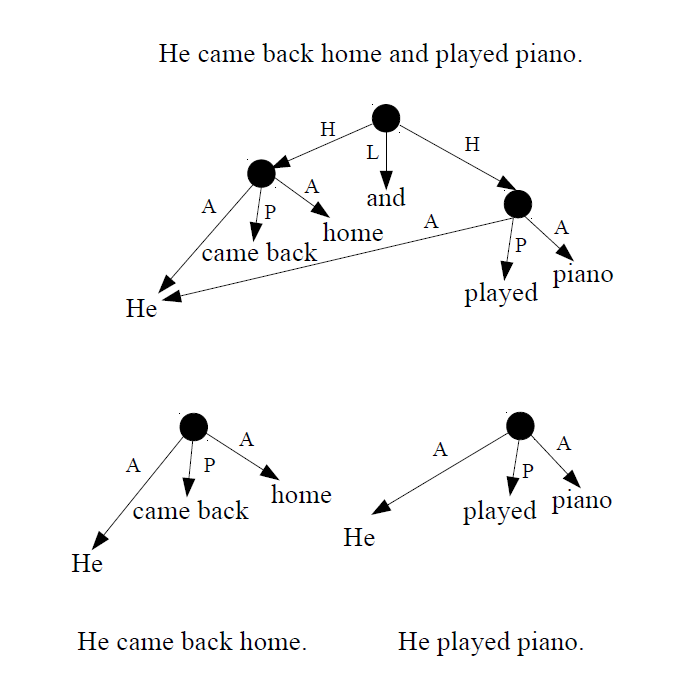
\includegraphics[width=1.2\textwidth,height=48mm]{ucca_simplification}  
    \end{minipage}
}
\end{frame}


\begin{frame}
\frametitle{Graph Structure}
UCCA structures are directed acyclic graphs (DAGs). \\
Text tokens are terminals, complex units are {\color{blue} non-terminal nodes}. \\
\textit{Remote edges} enable {\color{orange} reentrancy} for argument sharing. \\
Phrases may be {\color{red} discontinuous} (e.g., multi-word expressions).

\hspace*{1cm}
  \begin{tikzpicture}[level distance=16mm, sibling distance=2cm, ->,
  level 2/.style={level distance=9mm, sibling distance=1cm},
  level 4/.style={level distance=14mm}]
  \tikzstyle{word} = [font=\rmfamily,color=black]
    \node (ROOT) [fill=blue, circle] {}
      child {node (You) [word] {You} edge from parent node[left] {\scriptsize $A$}}
      child {node [word] {want} edge from parent node[left] {\scriptsize $P$}}
      child {node (totakealongbath) [fill=blue, circle] {}
      {
        child {node [word] {to} edge from parent node[left] {\scriptsize $F$}}
        child {node (takealongbath) [fill=blue, circle] {}
        {
          child {node (takeabath) [fill=blue, circle] {}
          {
            child {node [word] {take} edge from parent node[above] {\scriptsize $C$}}
            child {node [word] {a} edge from parent node[right] {\scriptsize $F$}}
            child {node [word] (long) {long} edge from parent[draw=none]}
            child {node [word] {bath} edge from parent node[right] {\scriptsize $C$}}
          } edge from parent node[left] {\scriptsize $C$} }
        } edge from parent node[right] {\scriptsize $P$} }
      } edge from parent node[left] {\scriptsize $A$} }
      ;
    \draw[bend left,dashed,->,orange,very thick] (totakealongbath) to node [auto] {\scriptsize $A$} (You);
    \draw[bend left,->,red,very thick] (takealongbath) to node [auto] {\scriptsize $D$} (long);
    \node at (6,-0.4) {\Large ----- primary edge};
    \node at (6,-1.4) {\Large - - - remote edge};
\end{tikzpicture}
\begin{center}
  You want to take a long bath
\end{center}

\vspace{-26mm}
\begin{adjustbox}{margin=1pt,frame,scale=.9}
  \begin{tabular}{c>{\small\it}l}
      $P$ & process \\
      $A$ & participant \\
      $C$ & center \\
      $D$ & adverbial \\
      $F$ & function
  \end{tabular}
\end{adjustbox}
\end{frame}


\begin{frame}
\frametitle{Structural Properties}
\noindent
\centering
\begin{minipage}{.48\linewidth}{\centering
(1) non-terminal nodes

\scalebox{.8}{
  \begin{tikzpicture}[level distance=12mm, sibling distance=16mm, ->,
      every node/.append style={midway}]
    \node (ROOT) [fill=black, circle] {}
      child {node [fill=black, circle] {}
      {
        child {node {John} edge from parent node[left] {\scriptsize $C$}}
        child {node {and} edge from parent node[left] {\scriptsize $N$}}
        child {node {Mary} edge from parent node[left] {\scriptsize $C$}}
      } edge from parent node[left] {\scriptsize $A$} }
      child {node {went} edge from parent node[left] {\scriptsize $P$}}
      child {node {home} edge from parent node[left] {\scriptsize $A$}}
      ;
  \end{tikzpicture}
  }}
\end{minipage}
\hfill
\begin{minipage}{.48\linewidth}{\centering
(2) discontinuity

\scalebox{.8}{
  \begin{tikzpicture}[level distance=12mm, sibling distance=2cm, ->,
      every node/.append style={midway}]
    \node (ROOT) [fill=black, circle] {}
      child {node {John} edge from parent node[left] {\scriptsize $A$}}
      child {node [fill=black, circle] {}
      {
      	child {node {gave} edge from parent node[left] {\scriptsize $C$}}
      	child {node (everything) {everything} edge from parent[white]}
      	child {node {up} edge from parent node[left] {\scriptsize $C$}}
      } edge from parent node[right] {\scriptsize $P$} }
      ;
    \draw[bend right,->] (ROOT) to[out=-20, in=180] node [left] {\scriptsize $A$} (everything);
  \end{tikzpicture}
  }}
\end{minipage}

\vfill
(3) reentrancy

\scalebox{.8}{
  \begin{tikzpicture}[level distance=12mm, sibling distance=2cm, ->,
      every node/.append style={midway}]
    \node (ROOT) [fill=black, circle] {}
      child {node (John) {John} edge from parent node[left] {\scriptsize $A$}}
      child {node {decided} edge from parent node[left] {\scriptsize $P$}}
      child {node (totakeaquickshower) [fill=black, circle] {}
      {
        child {node {to} edge from parent node[left] {\scriptsize $F$}}
        child {node [fill=black, circle] {}
        {
          child {node {take} edge from parent node[left] {\scriptsize $C$}}
          child {node {a} edge from parent node[right] {\scriptsize $F$}}
          child {node (quick) {quick} edge from parent[white]}
          child {node {shower} edge from parent node[right] {\scriptsize $C$}}
        } edge from parent node[right] {\scriptsize $P$} }
      } edge from parent node[left] {\scriptsize $A$} }
      ;
    \draw[bend left,dashed,->] (totakeaquickshower) to node [auto] {\scriptsize $A$} (John);
    \draw[bend left,->] (totakeaquickshower) to node [auto] {\scriptsize $D$} (quick);
  \end{tikzpicture}}
\end{frame}


\begin{frame}
\frametitle{Data}
\begin{itemize}
 \item UCCA Wikipedia corpus ($\stackrel{\text{train}}{4268}+\stackrel{\text{dev}}{454}+\stackrel{\text{test}}{503}$ sentences).
 \item Out-of-domain: English part of English-French parallel corpus,
     \textit{Twenty Thousand Leagues Under the Sea} (506 sentences).
\end{itemize}

\vfill
\begin{center}
  
\includegraphics[width=.5\linewidth]{wikipedia.png}
  
\includegraphics[width=.5\linewidth]{squid.jpg}
\end{center}
\end{frame}


\begin{frame}
\frametitle{UCCA Corpora}
\centering
\begin{tabular}{l|ccc|c}
    & \multicolumn{3}{c|}{Wiki} & 20K \\
    & \small Train & \small Dev & \small Test & Leagues \\
    \hline
    \# passages & 300 & 34 & 33 & 154 \\
    \# sentences & 4268 & 454 & 503 & 506 \\
    \hline
    \# nodes & 298,993 & 33,704 & 35,718 & 29,315 \\
    \% terminal & 42.96 & 43.54 & 42.87 & 42.09 \\
    \% non-term. & 58.33 & 57.60 & 58.35 & 60.01 \\
    \% \textbf{discont.} & \textbf{0.54} & \textbf{0.53} & \textbf{0.44} & \textbf{0.81} \\
    \% \textbf{reentrant} & \textbf{2.38} & \textbf{1.88} & \textbf{2.15} & \textbf{2.03} \\
    \hline
    \# edges & 287,914 & 32,460 & 34,336 & 27,749 \\
    \% primary & 98.25 & 98.75 & 98.74 & 97.73 \\
    \% remote & 1.75 & 1.25 & 1.26 & 2.27 \\
    \hline
    \multicolumn{3}{l}{\footnotesize Average per non-terminal node} \\
    \# children & 1.67 & 1.68 & 1.66 & 1.61 
\end{tabular}
\captionof{table}{Corpus statistics.}
\end{frame}



\section{Transition-based UCCA Parsing (ACL'17)}

\begin{frame}
\frametitle{Transition-Based Parsing}
First used for dependency parsing \cite{nivre2004incrementality}.

Parse text $w_1 \ldots w_n$ to graph $G$ incrementally by applying transitions to the parser state:
stack, buffer and constructed graph.

\pause
\vfill
Initial state:
\begin{tikzpicture}[every node/.append style={font=\rmfamily}, circle]
    \draw[xstep=1cm,ystep=5mm,color=gray] (-0.01,0) grid (1,.5);
    \node[anchor=west,style={font=\sffamily}] at (-0.1,1.00)     {stack};
    \node[fill=black] at (0.5,0.25) {};
    \draw[xstep=1cm,ystep=5mm,color=gray] (3,0) grid (10,.5);
    \node[anchor=west,style={font=\sffamily}] at (8.9,1.00) {buffer};
    \node[anchor=west] at (3,0.25) {\small You};
    \node[anchor=west] at (4,0.25) {\small want};
    \node[anchor=west] at (5,0.25) {\small to};
    \node[anchor=west] at (6,0.25) {\small take};
    \node[anchor=west] at (7,0.25) {\small a};
    \node[anchor=west] at (8,0.25) {\small long};
    \node[anchor=west] at (9,0.25) {\small bath};
\end{tikzpicture}

\vfill
\pause
\parser{} transitions:

\{\textsc{Shift, Reduce, Node$_X$, Left-Edge$_X$, Right-Edge$_X$,}\\
\hspace{5mm}\textsc{Left-Remote$_X$, Right-Remote$_X$, Swap, Finish}\}

\vfill
Support {\color{blue}non-terminal nodes}, {\color{orange}reentrancy} and {\color{red}discontinuity}.
\end{frame}

\begin{frame}
\frametitle{Example}
\begin{minipage}[t][8mm][t]{\textwidth}
    $\Rightarrow$\textsc{
        \only<1>{Shift}\only<2>{Right-Edge$_A$}\only<3>{Shift}\only<4>{Swap}\only<5>{Right-Edge$_P$}\only<6>{Reduce}\only<7>{Shift}\only<8>{Shift}\only<9>{Node$_F$}\only<10>{Reduce}\only<11>{Shift}\only<12>{Left-Remote$_A$}\only<13>{Shift}\only<14>{Node$_C$}\only<15>{Reduce}\only<16>{Shift}\only<17>{Right-Edge$_P$}\only<18>{Shift}\only<19>{Right-Edge$_F$}\only<20>{Reduce}\only<21>{Shift}\only<22>{Swap}\only<23>{Right-Edge$_D$}\only<24>{Reduce}\only<25>{Swap}\only<26>{Right-Edge$_A$}\only<27>{Reduce}\only<28>{Reduce}\only<29>{Shift}\only<30>{Reduce}\only<31>{Shift}\only<32>{Right-Edge$_C$}\only<33>{Finish}
    }
\end{minipage}

\vfill

\begin{tikzpicture}[every node/.append style={font=\rmfamily}]
    \only<31>\draw[xstep=1cm,ystep=5mm,color=red,line width=1pt] (-0.01,0) grid (1,.5);
    \only<1,7>\draw[xstep=1cm,ystep=5mm,color=red,line width=1pt] (.99,0) grid (2,.5);
    \only<2,5,26>\draw[xstep=1cm,ystep=5mm,color=red,line width=1pt] (-0.01,0) grid (2,.5);
    \only<3,8,11>\draw[xstep=1cm,ystep=5mm,color=red,line width=1pt] (1.99,0) grid (3,.5);
    \only<13,16>\draw[xstep=1cm,ystep=5mm,color=red,line width=1pt] (2.99,0) grid (4,.5);
    \only<18,21>\draw[xstep=1cm,ystep=5mm,color=red,line width=1pt] (3.99,0) grid (5,.5);
    \only<17>\draw[xstep=1cm,ystep=5mm,color=red,line width=1pt] (1.99,0) grid (4,.5);
    \only<19>\draw[xstep=1cm,ystep=5mm,color=red,line width=1pt] (2.99,0) grid (5,.5);
    \only<4>\draw[xstep=1cm,ystep=5mm,color=red,line width=1pt] (4,0) grid (5,.5);
    \only<9>\draw[xstep=1cm,ystep=5mm,color=red,line width=1pt] (5,0) grid (6,.5);
    \only<14>\draw[xstep=1cm,ystep=5mm,color=red,line width=1pt] (6,0) grid (7,.5);
    \only<22>\draw[xstep=1cm,ystep=5mm,color=red,line width=1pt] (8,0) grid (9,.5);
    \only<25>\draw[xstep=1cm,ystep=5mm,color=red,line width=1pt] (7,0) grid (8,.5);
    \only<23>\draw[xstep=1cm,ystep=5mm,color=red,line width=1pt] (1.99,0) grid (4,.5);
    \only<32>\draw[xstep=1cm,ystep=5mm,color=red,line width=1pt] (-0.01,0) grid (2,.5);
    \only<12>\draw[xstep=1cm,ystep=5mm,color=red,line width=1pt] (.99,0) grid (3,.5);
    \only<28,30>\draw[xstep=1mm,ystep=5mm,color=gray] (-0.01,0) grid (0.1,.5);
    \only<6,27,29,31->\draw[xstep=1cm,ystep=5mm,color=gray] (-0.01,0) grid (1,.5);
    \only<-2,4-5,7,10,25-26,33>\draw[xstep=1cm,ystep=5mm,color=gray] (-0.01,0) grid (2,.5);
    \only<3,8-9,11-12,15,24>\draw[xstep=1cm,ystep=5mm,color=gray] (-0.01,0) grid (3,.5);
    \only<13-14,16-17,20,22-23>\draw[xstep=1cm,ystep=5mm,color=gray] (-0.01,0) grid (4,.5);
    \only<18-19,21>\draw[xstep=1cm,ystep=5mm,color=gray] (-0.01,0) grid (5,.5);
    \node[anchor=west,style={font=\sffamily}] at (-0.1,1.00){stack};
    \only<-27>\node[fill=black, circle] at (0.5,0.25) {};
    \only<25-26> \node[fill=blue, circle] at (1.5,0.25) {};
    \only<11-24> \node[fill=blue, circle] at (2.5,0.25) {};
    \only<31-> \node[fill=red, circle] at (0.5,0.25) {};
    \only<16-21> \node[fill=red, circle] at (3.5,0.25) {};
    \only<29> \node[anchor=west] at (0,0.25) {\small You};
    \only<1-3,7-24> \node[anchor=west] at (1,0.25) {\small You};
    \only<4-5> \node[anchor=west] at (1,0.25) {\small want};
    \only<3>   \node[anchor=west] at (2,0.25) {\small want};
    \only<8-9>  \node[anchor=west] at (2,0.25) {\small to};
    \only<13-14> \node[anchor=west] at (3,0.25) {\small take};
    \only<18-19> \node[anchor=west] at (4,0.25) {\small a};
    \only<21> \node[anchor=west] at (4,0.25) {\small long};
    \only<22-23> \node[anchor=west] at (3,0.25) {\small long};
    \only<32-> \node[anchor=west] at (1,0.25) {\small bath};
    \only<-2,4-6>\draw[xstep=1cm,ystep=5mm,color=gray] (4,0) grid (10,.5);
    \only<3,5-7,9-10>\draw[xstep=1cm,ystep=5mm,color=gray] (5,0) grid (10,.5);
    \only<8,11-12,14-15>\draw[xstep=1cm,ystep=5mm,color=gray] (6,0) grid (10,.5);
    \only<13,16-17,25-28>\draw[xstep=1cm,ystep=5mm,color=gray] (7,0) grid (10,.5);
    \only<18-20,22-24,29-30>\draw[xstep=1cm,ystep=5mm,color=gray] (8,0) grid (10,.5);
    \only<21,31>\draw[xstep=1cm,ystep=5mm,color=gray] (9,0) grid (10,.5);
    \only<32->\draw[xstep=1mm,ystep=5mm,color=gray] (9.89,0) grid (10,.5);
    \node[anchor=west,style={font=\sffamily}] at (8.9,1) {buffer};
    \only<9-10> \node[fill=blue, circle] at (5.5,0.25) {};
    \only<14-15> \node[fill=red, circle] at (6.5,0.25) {};
    \only<22-30> \node[fill=red, circle] at (8.5,0.25) {};
    \only<4-6> \node[anchor=west] at (4,0.25) {\small You};
    \only<25-28> \node[anchor=west] at (7,0.25) {\small You};
    \only<-2>  \node[anchor=west] at (4,0.25) {\small want};
    \only<-7> \node[anchor=west] at (5,0.25) {\small to};
    \only<-12> \node[anchor=west] at (6,0.25) {\small take};
    \only<-17> \node[anchor=west] at (7,0.25) {\small a};
    \only<-20> \node[anchor=west] at (8,0.25) {\small long};
    \only<-31> \node[anchor=west] at (9,0.25) {\small bath};
\end{tikzpicture}
\vfill
\fbox{
\begin{tikzpicture}[level distance=15mm, sibling distance=2cm, ->,
    every node/.append style={font=\rmfamily}]
    \node[anchor=west,style={font=\sffamily}] at (0,0) {graph};
    \node(ROOT)[fill=black, circle, visible on=<1->] at (3,0) {}
      child [visible on=<2->,alt=<2>{draw=red}{}] {node (You) {You} edge from parent node [left] {\scriptsize $A$}}
      child [visible on=<5->,alt=<5>{draw=red}{}] {node (want) {want} edge from parent node [left] {\scriptsize $P$}}
      child [visible on=<9->] {node (totakealongbath) [fill=blue, circle] {}
      {
        child [visible on=<9->] {node (to) {to} edge from parent node [left] {\scriptsize $F$}}
        child [visible on=<14->] {node (takeabath) [fill=red, circle] {}
        {
          child [visible on=<14->] {node (take) {take} edge from parent node [right] {\scriptsize $C$}}
          child [visible on=<19->,alt=<19>{draw=red}{}] {node (a) {a} edge from parent node [right] {\scriptsize $F$}}
          child [visible on=<23->,alt=<23>{draw=red}{}] {node (long) {long} edge from parent [draw=none]}
          child [visible on=<32->,alt=<32>{draw=red}{}] {node (bath) {bath} edge from parent node [right] {\scriptsize $C$}}
        } edge from parent [draw=none]}
      } edge from parent [draw=none]}
      ;
    \draw[visible on=<17->,alt=<17>{draw=red}{}] (totakealongbath) to node [left] {\scriptsize $P$} (takeabath);
    \draw[visible on=<26->,alt=<26>{draw=red}{}] (ROOT) to node [left] {\scriptsize $A$} (totakealongbath);
    \draw[bend left,dashed, visible on=<12->,alt=<12>{draw=red}{}] (totakealongbath) to node [auto] {\scriptsize $A$} (You);
    \draw[bend left, visible on=<23->] (totakealongbath) to node [auto] {\scriptsize $D$} (long);
\end{tikzpicture}}
\end{frame}

\begin{frame}
\frametitle{Training}
An \textit{oracle} provides the transition sequence given the correct graph:

\vfill
\centering
\scalebox{.8}{
\begin{tikzpicture}[level distance=15mm, sibling distance=2cm, ->,
    every node/.append style={font=\rmfamily}]
    \node(ROOT)[fill=black, circle] at (3,0) {}
      child {node (You) {You} edge from parent node [left] {\scriptsize $A$}}
      child {node (want) {want} edge from parent node [left] {\scriptsize $P$}}
      child {node (totakealongbath) [fill=blue, circle] {} 
      { 
        child {node (to) {to} edge from parent node [left] {\scriptsize $F$}}
        child {node (takeabath) [fill=red, circle] {}
        {
          child {node (take) {take} edge from parent node [right] {\scriptsize $C$}}      
          child {node (a) {a} edge from parent node [right] {\scriptsize $F$}} 
          child {node (long) {long} edge from parent [draw=none]}
          child {node (bath) {bath} edge from parent node [right] {\scriptsize $C$}}  
        } edge from parent [draw=none]}
      } edge from parent [draw=none]}
      ;
    \draw(totakealongbath) to node [left] {\scriptsize $P$} (takeabath); 
    \draw(ROOT) to node [left] {\scriptsize $A$} (totakealongbath);
    \draw[bend left,dashed] (totakealongbath) to node [auto] {\scriptsize $A$} (You);
    \draw[bend left] (totakealongbath) to node [auto] {\scriptsize $D$} (long);
\end{tikzpicture}}
\[\Downarrow\]
\begin{flushleft}
\footnotesize
\textsc{Shift}, \textsc{Right-Edge$_A$}, \textsc{Shift}, \textsc{Swap}, \textsc{Right-Edge$_P$}, \textsc{Reduce}, \textsc{Shift}, \textsc{Shift}, \textsc{Node$_F$}, \textsc{Reduce}, \textsc{Left-Remote$_A$}, \textsc{Shift}, \textsc{Shift}, \textsc{Node$_C$}, \textsc{Reduce}, \textsc{Shift}, \textsc{Right-Edge$_P$}, \textsc{Shift}, \textsc{Right-Edge$_F$}, \textsc{Reduce}, \textsc{Shift}, \textsc{Swap}, \textsc{Right-Edge$_D$}, \textsc{Reduce}, \textsc{Swap}, \textsc{Right-Edge$_A$}, \textsc{Reduce}, \textsc{Reduce}, \textsc{Shift}, \textsc{Reduce}, \textsc{Shift}, \textsc{Right-Edge$_C$}, \textsc{Finish}
\end{flushleft}
\end{frame}

\begin{frame}
\only<-5>{
\frametitle{\parser{} Model}
Learn to greedily predict transition based on current state.

Experimenting with three classifiers:
\vspace{5mm}

    \begin{tabular}{ll}
    \textbf{Sparse} & Perceptron with sparse features \cite{ZhangTDP11}. \\
    \textbf{MLP} & Embeddings + feedforward NN \cite{chen2014fast}. \\
    \textbf{BiLSTM} & Embeddings + \only<2->{\textbf}{deep bidirectional LSTM} + MLP \\&
    \cite{kiperwasser2016simple}.
    \onslide<2>{\\ \\& Effective ``lookahead'' encoded in the representation.}
    \end{tabular}
}
\only<2-5>{\vspace{-53mm}}

\only<1>{
\vfill

Features:
words, POS, syntactic dependencies, existing edge labels \\
from the stack and buffer + parents, children, grandchildren;
ordinal features (height, number of parents and children)

\vspace{5mm}
\begin{tikzpicture}
    \draw[xstep=1cm,ystep=5mm,color=gray] (-0.01,0) grid (4,.5);
    \draw[xstep=1cm,ystep=5mm,color=gray] (5,0) grid (10,.5);
    \node[anchor=west] at (-0.1,1.00) {stack};
    \node[anchor=west] at (8.9,1.00) {buffer};
    \foreach \i in {0.5,8.5,9.5} {
        \node[fill=gray, circle] at (\i,0.25) {};
    }
    \foreach \i in {1.5,2.5,3.5,5.5,6.5,7.5} {
        \node[fill=black, circle] at (\i,0.25) {};
    }
\end{tikzpicture}
}
\centering
\onslide<6>{
\fbox{
\begin{minipage}{.5\textwidth}
\begin{tikzpicture}[every node/.append style={font=\rmfamily}]
    \node[anchor=west,style={font=\sffamily}] at (-1.2,0.25){stack};
    \draw[xstep=1cm,ystep=5mm,color=gray] (-0.01,0) grid (4,.5);
    \node[fill=black, circle] at (0.5,0.25) {};
    \node[fill=blue, circle] at (2.5,0.25) {};
    \node[anchor=west] at (1,0.25) {\small You};
    \node[anchor=west] at (3,0.25) {\small take};
\end{tikzpicture}

\vspace{1cm}
\begin{tikzpicture}[every node/.append style={font=\rmfamily}]
    \node[anchor=west,style={font=\sffamily}] at (3.8,0.25){buffer};
    \draw[xstep=1cm,ystep=5mm,color=gray] (5,0) grid (9,.5);
    \node[fill=red, circle] at (5.5,0.25) {};
    \node[anchor=west] at (6,0.25) {\small a};
    \node[anchor=west] at (7,0.25) {\small long};
    \node[anchor=west] at (8,0.25) {\small bath};
\end{tikzpicture}
\end{minipage}
\begin{minipage}{.4\textwidth}
\scalebox{.8}{
\begin{tikzpicture}[level distance=1cm, sibling distance=1cm, ->,
    every node/.append style={font=\rmfamily}]
    \node[anchor=west,style={font=\sffamily}] at (5,0) {graph};
    \draw[color=gray] (1.2,.3) rectangle (4.9,-3.2);
    \node(ROOT)[fill=black, circle, visible on=<2->] at (3,0) {}
      child {node (You) {You} edge from parent node [left] {\scriptsize $A$}}
      child {node {want} edge from parent node [left] {\scriptsize $P$}}
      child {node (totakealongbath) [fill=blue, circle] {}
      {
        child {node {to} edge from parent node [left] {\scriptsize $F$}}
        child {node (takeabath) [fill=red, circle] {}
        {
          child {node {take} edge from parent node [right] {\scriptsize $C$}}
          child [opacity=0] {node {a} edge from parent node [right] {\scriptsize $F$}}
          child [opacity=0] {node (long) {long} edge from parent [draw=none]}
          child [opacity=0] {node {bath} edge from parent node [right] {\scriptsize $C$}}
        } edge from parent [draw=none]}
      } edge from parent [draw=none]}
      ;
\end{tikzpicture}
}
\end{minipage}
}
}
\onslide<2->{
\scalebox{.7}{
\begin{tikzpicture}[->]
    \tiny
    \tikzstyle{main}=[circle, minimum size=7mm, draw=black!80, node distance=12mm]
    \foreach \i/\word in {1/{You},3/{want},5/{to},7/{take},9/{a},11/{long},13/{bath}} {
        \onslide<2->\node (x\i) at (\i,-1.3) {\Large\textrm\word};
        \onslide<2->\node[main, fill=white!100] (h\i) at (\i,0) {LSTM};
        \onslide<2->\path (x\i) edge (h\i);
        \onslide<3->\node[main, fill=white!100] (i\i) at (\i.5,.8) {LSTM};
        \onslide<3->\path (x\i) edge [bend right] (i\i);
        \onslide<4->\node[main, fill=white!100] (l\i) at (\i.5,2.3) {LSTM};
        \onslide<4->\path (h\i) edge [bend left] (l\i);
        \onslide<4->\path (i\i) edge (l\i);
        \onslide<5->\node[main, fill=white!100] (k\i) at (\i,3.1) {LSTM};
        \onslide<5->\path (i\i) edge [bend left] (k\i);
        \onslide<5->\path (h\i) edge [bend left] (k\i);
    }
    \foreach \current/\next in {1/3,3/5,5/7,7/9,9/11,11/13} {
        \onslide<2->\path (h\current) edge (h\next);
        \onslide<3->\path (i\next) edge (i\current);
        \onslide<4->\path (l\current) edge (l\next);
        \onslide<5->\path (k\next) edge (k\current);
    }
    \onslide<6>\node[main, fill=white!100] (mlp) at (7,4.6) {MLP};
    \onslide<6>\foreach \i in {5,7,9} {
        \path (l\i) edge (mlp);
        \path (k\i) edge (mlp);
    }
    \coordinate (state) at (10.5,6.5);
    \onslide<6>\path (state) edge [bend left] (mlp);
    \onslide<6>\node (transition) at (7,5.8) {\large\textsc{Node}$_C$};
    \onslide<6>\path (mlp) edge (transition);
\end{tikzpicture}
}
}
\end{frame}

\begin{frame}
\frametitle{Baselines}
No existing UCCA parsers $\Rightarrow$ conversion-based approximation.

\vfill
\footnotesize
Bi-lexical DAG parsers (allow {\color{orange}reentrancy}):
\begin{itemize}
 \item DAGParser \cite{ribeyre-villemontedelaclergerie-seddah:2014:SemEval}:
 transition-based.
 \item TurboParser \cite{almeida-martins:2015:SemEval}:
 graph-based.
\end{itemize}

Tree parsers (all transition-based):
\begin{itemize}
 \item MaltParser \cite{nivre2007maltparser}: bi-lexical tree parser.
 \item Stack LSTM Parser \cite{dyer2015transition}: bilexical tree parser.
 \item \textsc{uparse} \cite{maier2015discontinuous}: allows {\color{blue}non-terminals}, {\color{red}discontinuity}.
\end{itemize}

\vfill
\begin{center}
    \begin{dependency}
    \begin{deptext}[column sep=1.5em,ampersand replacement=\^,font=\rmfamily]
	You \^ want \^ to \^ take \^ a \^ long \^ bath \\
    \end{deptext}
    \depedge{2}{1}{$A$}
    \depedge{2}{4}{$A$}
    \depedge[dashed,edge start x offset=6pt]{4}{1}{$A$}
    \depedge{4}{3}{$F$}
    \depedge{4}{5}{$F$}
    \depedge{4}{6}{$D$}
    \depedge{4}{7}{$C$}
    \end{dependency}
    \captionof{figure}{UCCA bilexical DAG approximation (for tree, delete remote edges).}
\end{center}
\end{frame}


\begin{frame}
\frametitle{Bilexical Graph Approximation}
\begin{enumerate}
 \item Convert UCCA to bilexical dependencies.
 \item Train bilexical parsers and apply to test sentences.
 \item Reconstruct UCCA graphs and compare with gold standard.
\end{enumerate}
\vfill

\begin{flushright}
    \begin{tikzpicture}[level distance=13mm, sibling distance=17mm, ->,
        every circle node/.append style={fill=black}]
      \tikzstyle{word} = [font=\rmfamily,color=black]
      \node (ROOT) [circle] {}
        child {node (After) [word] {After} edge from parent node[left] {\scriptsize $L$}}
        child {node (graduation) [circle] {}
        {
          child {node [word] {graduation} edge from parent node[left] {\scriptsize $P$}}
        } edge from parent node[left] {\scriptsize $H$} }
        child {node [word] {,} edge from parent node[right] {\scriptsize $U$}}
        child {node (moved) [circle] {}
        {
          child {node (Joe) [word] {Joe} edge from parent node[left] {\scriptsize $A$}}
          child {node [word] {moved} edge from parent node[left] {\scriptsize $P$}}
          child {node [circle] {}
          {
            child {node [word] {to} edge from parent node[left] {\scriptsize $R$}}
            child {node [word] {Copenhagen} edge from parent node[right] {\scriptsize $C$}}
          } edge from parent node[right] {\scriptsize $A$} }
        } edge from parent node[right] {\scriptsize $H$} }
        ;
      \draw[dashed,->] (graduation) to node [auto] {\scriptsize $A$} (Joe);
    \end{tikzpicture}
\end{flushright}

\vspace{-14mm}
\begin{flushleft}
    \begin{dependency}
    \begin{deptext}[column sep=.7em,ampersand replacement=\^,font=\rmfamily]
	After \^ graduation \^ , \^ Joe \^ moved \^ to \^ Copenhagen \\
    \end{deptext}
    \depedge{2}{1}{$L$}
    \depedge{2}{3}{$U$}
    \depedge[dashed]{2}{4}{$A$}
    \depedge{5}{4}{$A$}
    \depedge{2}{5}{$H$}
    \depedge{7}{6}{$R$}
    \depedge{5}{7}{$A$}
    \end{dependency}
\end{flushleft}
\end{frame}

\begin{frame}
\frametitle{Evaluation}
\textit{Mutual edges} between predicted graph $G_p=(V_p,E_p,\ell_p)$
and gold graph $G_g=(V_g,E_g,\ell_g)$,
both over terminals $W = \{w_1,\ldots,w_n\}$:
\[
M(G_p,G_g) =
    \Bigl\{(e_1,e_2) \in E_p \times E_g \;\Big|\;
    y(e_1) = y(e_2) \wedge \ell_p(e_1)=\ell_g(e_2)\Bigr\}
\]
The yield $y(e) \subseteq W$ of an edge $e=(u,v)$ in either graph
is the set of terminals in $W$ that are descendants of $v$. \hfill
$\ell$ is the edge label.

\vfill
Labeled precision, recall and F-score are then defined as:
\[
\text{LP} = \frac{|M(G_p,G_g)|}{|E_p|},\quad
\text{LR} = \frac{|M(G_p,G_g)|}{|E_g|},
\]
\[
\text{LF} = \frac{2 \cdot \text{LP} \cdot \text{LR}}{\text{LP} + \text{LR}}.
\]
Two variants:
one for primary edges, and another for remote edges.
\end{frame}


\begin{frame}
\frametitle{Evaluation}
Comparing graphs over the same sequence of tokens,
\begin{itemize}
\item Match edges by their terminal yield and label.
\item Calculate \textbf{labeled precision, recall and F1} scores.
\item Separate primary and remote edges.
\end{itemize}
\vfill
\begin{adjustbox}{frame,scale=.75,center}
    \begin{tikzpicture}[level distance=15mm, sibling distance=15mm, ->,
        every circle node/.append style={fill=black}]
      \tikzstyle{word} = [font=\rmfamily,color=black]
      \node at (-1,.7) {gold};
      \node (ROOT) at (0,0) [circle] {}
        child {node (After) [word] {After} edge from parent node[left] {$L$}}
        child {node (graduation) [circle] {}
        {
          child {node [word] {graduation} edge from parent node[left] {$P$}}
        } edge from parent node[left] {$H$} }
        child {node [word] {,} edge from parent node[right] {$U$}}
        child {node (moved) [circle] {}
        {
          child {node (Joe) [word] {Joe} edge from parent node[left] {$A$}}
          child {node [word] {moved} edge from parent node[left] {$P$}}
          child {node [circle] {}
          {
            child {node [word] {to} edge from parent node[left] {$R$}}
            child {node [word] {Copenhagen} edge from parent node[right] {$C$}}
          } edge from parent node[right] {$A$} }
        } edge from parent node[right] {$H$} }
        ;
      \draw[dashed,->] (graduation) to node [auto] {$A$} (Joe);
      \node at (6,.7) {predicted};
      \node (ROOT_) at (7,0) [circle] {}
        child {node (After_) [word] {After} edge from parent node[left] {$L$}}
        child {node (graduation_) [circle] {}
        {
          child[red] {node [word] {graduation} edge from parent node[left] {$S$}}
        } edge from parent node[left] {$H$} }
        child {node [word] {,} edge from parent node[right] {$U$}}
        child {node (moved) [circle,xshift=3mm,yshift=-7mm] {}
        {
          child {node (Joe_) [word] {Joe} edge from parent node[left] {$A$}}
          child {node [word] {moved} edge from parent node[left] {$P$}}
          child[red] {node [word] {to} edge from parent node[left] {$F$}}
          child[red] {node (Copenhagen_) [word] {Copenhagen} edge from parent node[right] {$A$}}
        } edge from parent node[right] {$H$} }
        ;
      \draw[bend left,dashed,->] (graduation_) to node [auto] {$A$} (Joe_);
      \draw[bend left,dashed,->,red] (graduation_) to node [auto] {$A$} (Copenhagen_);
    \end{tikzpicture}
\end{adjustbox}
\vfill
\begin{adjustbox}{scale=.75,center}
	Primary:
    \begin{tabular}{ccc}
        \textbf{LP} & \textbf{LR} & \textbf{LF} \\ \hline
        $\frac69=67\%$ & $\frac6{10}=60\%$ & 64\%
    \end{tabular}
    \hspace{1cm}
	Remote:
    \begin{tabular}{ccc}
        \textbf{LP} & \textbf{LR} & \textbf{LF} \\ \hline
        $\frac12=50\%$ & $\frac11=100\%$ & 67\%
    \end{tabular}
\end{adjustbox}
\end{frame}


\begin{frame}
\frametitle{Results}
\parser{BiLSTM} obtains the highest F-scores in all metrics:
\begin{center}
    \begin{tabular}{l|ccc|ccc}
        & \multicolumn{3}{c|}{Primary edges} & \multicolumn{3}{c}{Remote edges} \\
        & \textbf{LP} & \textbf{LR} & \textbf{LF} & \textbf{LP} & \textbf{LR} & \textbf{LF} \\
        \hline
        \parser{Sparse}
        & 64.5 & 63.7 & 64.1 & 19.8 & 13.4 & 16 \\
        \parser{MLP}
        & 65.2 & 64.6 & 64.9 & 23.7 & 13.2 & 16.9 \\
        \parser{BiLSTM}
        & 74.4 & 72.7 & \textbf{73.5} & 47.4 & 51.6 & \textbf{49.4} \\
        \hline
        \scriptsize Bilexical DAG
        & & & \scriptsize (91) & & & \scriptsize (58.3) \\
    	DAGParser
        & 61.8 & 55.8 & 58.6 & 9.5 & 0.5 & 1 \\
    	TurboParser
        & 57.7 & 46 & 51.2 & 77.8 & 1.8 & 3.7 \\
        \hline
        \scriptsize Bilexical tree
        & & & \scriptsize (91) & & & \scriptsize -- \\
    	MaltParser
        & 62.8 & 57.7 & 60.2 & -- & -- & -- \\
    	Stack LSTM
        & 73.2 & 66.9 & 69.9 & -- & -- & -- \\
        \hline
        \scriptsize Tree
        & & & \scriptsize (100) & & & \scriptsize -- \\
        \textsc{uparse}
        & 60.9 & 61.2 & 61.1 & -- & -- & --
    \end{tabular}
    \captionof{table}{Results on the Wiki test set.}
\end{center}
\end{frame}


\begin{frame}
\frametitle{Results}
Comparable on out-of-domain test set:
\begin{center}
    \begin{tabular}{l|ccc|ccc}
        & \multicolumn{3}{c|}{Primary edges} & \multicolumn{3}{c}{Remote edges} \\
        & \textbf{LP} & \textbf{LR} & \textbf{LF} & \textbf{LP} & \textbf{LR} & \textbf{LF} \\
        \hline
        \parser{Sparse}
        & 59.6 & 59.9 & 59.8 & 22.2 & 7.7 & 11.5 \\
        \parser{MLP}
        & 62.3 & 62.6 & 62.5 & 20.9 & 6.3 & 9.7 \\
        \parser{BiLSTM}
        & 68.7 & 68.5 & \textbf{68.6} & 38.6 & 18.8 & \textbf{25.3} \\
        \hline
        \scriptsize Bilexical DAG
        & & & \scriptsize (91.3) & & & \scriptsize (43.4) \\
    	DAGParser
        & 56.4 & 50.6 & 53.4 & -- & 0 & 0 \\
    	TurboParser
        & 50.3 & 37.7 & 43.1 & 100 & 0.4 & 0.8 \\
        \hline
        \scriptsize Bilexical tree
        & & & \scriptsize (91.3) & & & \scriptsize -- \\
    	MaltParser
        & 57.8 & 53 & 55.3 & -- & -- & -- \\
    	Stack LSTM
        & 66.1 & 61.1 & 63.5 & -- & -- & -- \\
        \hline
        \scriptsize Tree
        & & & \scriptsize (100) & & & \scriptsize -- \\
        \textsc{uparse}
        & 52.7 & 52.8 & 52.8 & -- & -- & --
    \end{tabular}
    \captionof{table}{Results on the 20K Leagues out-of-domain set.}
\end{center}
\end{frame}


\begin{frame}
\frametitle{TUPA}
\begin{tikzpicture}[every node/.append style={font=\rmfamily}, circle]
    \node[anchor=west,style={font=\sffamily}] at (-1,.25)     {State:};
    \draw[xstep=1cm,ystep=5mm,color=gray] (1,0) grid (2,.5);
    \node[anchor=west,style={font=\sffamily}] at (.9,.75)     {stack};
    \node[fill=black] at (1.5,0.25) {};
    \draw[xstep=12.5mm,ystep=5mm,color=gray] (2.5,0) grid (10,.5);
    \node[anchor=west,style={font=\sffamily}] at (2.4,.75) {buffer};
    \node[anchor=west] at (2.5,0.25) {\small After};
    \node[anchor=west] at (3.75,0.25) {\small gradu.};
    \node[anchor=west] at (5,0.25) {\small John};
    \node[anchor=west] at (6.25,0.25) {\small moved};
    \node[anchor=west] at (7.5,0.25) {\small to};
    \node[anchor=west] at (8.75,0.25) {\small Copenhagen};
\end{tikzpicture}

\vfill
\pause
Transitions:

\{\textsc{Shift, Reduce, Node$_X$, Left-Edge$_X$, Right-Edge$_X$,}\\
\hspace{5mm}\textsc{Left-Remote$_X$, Right-Remote$_X$, Swap, Finish}\}

\vfill
\pause
Classifier:
\vspace{-2.5mm}
    \begin{center}\scalebox{.3}{\Huge
       \begin{tikzpicture}[-{Latex[length=3mm]},thick]
       \tikzstyle{main}=[rounded rectangle, minimum size=15mm, draw=black!80, node distance=12mm]
       \node[main] (specific) at (10.5,12.5) {BiLSTM};
       \foreach \i/\word in {-4/{After},4/{graduation},17/{to},25/{Copenhagen}} {
           \node (x\i) at (\i,8.5) {\word};
           \node[main, minimum size=8mm, fill=black, draw=none] (e\i) at (\i,10.5) {};
           \path (x\i) edge (e\i);
           \path (e\i) edge (specific);
       }
        \node (x4) at (10.5,8.5) {\ldots};
        \node[main] (state) at (20,15) {state};
        \node[main] (mlp) at (10.5,15) {MLP};
        \path (specific) edge (mlp);
        \path (state) edge node[below] {concatenate} (mlp);
        \node (transition) at (10.5,17.8) {transition};
        \path (mlp) edge node[right] {softmax} (transition);
       \end{tikzpicture}}
    \end{center}
\end{frame}

\begin{frame}
\frametitle{Results}
\centering
\small
\setlength\tabcolsep{3pt}
\begin{tabular}{lcc}
& \footnotesize \bf Primary F1 & \footnotesize \bf Remote F1 \\
\hline
\small \bf English (in-domain)     & 73.6 & 51.5 \\
\small \bf English (out-of-domain) & 69.0 & 26.7 \\
\small \bf French (in-domain)      & 67.6 & 13.9 \\
\small \bf German (in-domain)      & 72.5 & 27.1
\end{tabular}
\vfill

\begin{center}
  \begin{minipage}{.3\textwidth}
\includegraphics[width=\textwidth]{wikipedia.png}\end{minipage}
  \begin{minipage}{.3\textwidth}
\includegraphics[width=\textwidth]{squid.jpg}\end{minipage}
\end{center}
\end{frame}



\section{Multitask Parsing across Semantic Representations (ACL'18)}

\semanticrepresentations

\begin{frame}
    \frametitle{Data}
    \fbox{UCCA training data is scarce}
    \begin{center}
    \pgfplotstableread[row sep=\\,col sep=&]{
    	corpus & total \\
        \color{DarkBlue} \textbf{UD} & 17062 \\
        \color{DarkRed} \textbf{SDP} & 33964 \\
        \color{DarkGreen} \textbf{AMR} & 36521 \\
        \color{Indigo} \textbf{UCCA} & 5225 \\
        }\english
        \begin{tikzpicture}
        \begin{axis}[
        xbar stacked,
        width=10cm,
        height=39mm,
        xmin=0,
        xmax=60000,
        xtick=\empty,
        ytick=data,
        yticklabels from table={\english}{corpus},
        axis x line=none,
        ]
        \addplot [fill=Navy, point meta=explicit symbolic,
        nodes near coords={\pgfmathprintnumber\pgfplotspointmeta~sentences},
        nodes near coords align={anchor=west}] table [x=total,y expr=\coordindex,meta=total] {\english};
        \end{axis}
        \end{tikzpicture}
    \end{center}
    
    \pause
    \vfill
    
    \begin{flushright}
        \fbox{and domains are limited.}
    \end{flushright}
    \begin{center}
    \begin{tabular}{llll}
        \color{Indigo} \textbf{UCCA}  & \color{DarkGreen} \textbf{AMR}  & \color{DarkRed} \textbf{SDP}  & \color{NavyBlue} \textbf{UD}  \\
    	Wikipedia & blogs & news & blogs \\ books & news && news \\ & emails && emails \\ & reviews && reviews \\ &&& Q\&A
    \end{tabular}
    \end{center}
\end{frame}


\begin{frame}
\frametitle{Conversion}

\begin{minipage}{.04\textwidth}
\vspace{4mm}
AMR\\
\vspace{13mm}
SDP\\
\vspace{14mm}
UD
\end{minipage}
\begin{minipage}{.45\textwidth}
  \centering
  \scalebox{.6}{
  \begin{tikzpicture}[->,
      every node/.append style={sloped,anchor=south,auto=false,font=\tiny},
      level 1/.style={level distance=14mm,sibling distance=26mm},
      level 2/.style={level distance=13mm},
      level 3/.style={level distance=12mm}]
    \node (ROOT) [draw=black,ellipse] {move-01}
      child {node [draw=black,ellipse] {after}
      {
            child {node (graduation) [draw=black,ellipse] {graduate-01} edge from parent node {op1} }
      } edge from parent node {time} }
      child {node (John) [draw=black,ellipse] {person}
      {
        child {node [draw=black,ellipse] {name}
        {
            child {node [draw=black,ellipse] {"John"} edge from parent node {op1} }
        } edge from parent node {name} }
      } edge from parent node {ARG0} }
      child {node [draw=black,ellipse] {city}
      {
        child {node [draw=black,ellipse] {name}
        {
            child {node [draw=black,ellipse] {"Copenhagen"} edge from parent node {op1} }
        } edge from parent node {name} }
      } edge from parent node {ARG2} }
      ;
      \draw (graduation) to node {ARG0} (John);
  \end{tikzpicture}
  }
  
  \vspace{5mm}
  \scalebox{.6}{
    \begin{dependency}[text only label, label style={above}, font=\small]
    \begin{deptext}[column sep=.8em,ampersand replacement=\^]
    After \^ graduation \^ , \^ John \^ moved \^ to \^ Copenhagen \\
    \end{deptext}
        \depedge{1}{2}{ARG2}
        \depedge{5}{4}{ARG1}
        \depedge[edge end x offset=-2pt]{1}{5}{ARG1}
        \deproot[edge unit distance=3.5ex]{5}{top}
        \depedge[edge start x offset=-1pt, edge end x offset=3pt]{5}{7}{ARG2}
        \depedge[edge end x offset=5pt]{6}{5}{ARG1}
        \depedge{6}{7}{ARG2}
    \end{dependency}
    }
    
  \vspace{5mm}
  \scalebox{.6}{
    \begin{dependency}[text only label, label style={above}, font=\small]
    \begin{deptext}[column sep=.8em,ampersand replacement=\^]
    After \^ graduation \^ , \^ John \^ moved \^ to \^ Copenhagen \\
    \end{deptext}
        \depedge{2}{1}{case}
        \depedge{2}{3}{punct}
        \depedge{5}{4}{nsubj}
        \depedge[edge end x offset=-2pt]{5}{2}{obl}
        \depedge{7}{6}{case}
        \deproot[edge unit distance=2.5ex]{5}{root}
        \depedge{5}{7}{obl}
    \end{dependency}
    }

\end{minipage}
\begin{minipage}{.02\textwidth}
\vspace{7mm}
\Rightarrow
\vspace{16mm}
\Rightarrow
\vspace{20mm}
\Rightarrow
\end{minipage}
\begin{minipage}{.45\textwidth}

  \centering
  \scalebox{.6}{
  \begin{tikzpicture}[level distance=16mm, ->,
      every node/.append style={sloped,anchor=south,auto=false,font=\scriptsize},
      level 1/.style={sibling distance=28mm},
      level 2/.style={sibling distance=14mm},
      level 3/.style={sibling distance=12mm}]
    \tikzstyle{word} = [font=\rmfamily,color=black]
    \node (ROOT) [word] {moved}
      child {node [word] {After}
      {
            child {node (graduation) [word] {graduation} edge from parent node {op} }
      } edge from parent node {time} }
      child {node (John) [fill=black,circle] {}
      {
        child {node [word] {John} edge from parent node {name} }
      } edge from parent node {ARG0} }
      child {node [fill=black,circle] {}
      {
        child {node [word] {Copenhagen} edge from parent node {name} }
      } edge from parent node {ARG2} }
      ;
      \draw[dashed] (graduation) to node {ARG0} (John);
  \end{tikzpicture}}

  \vspace{5mm}
  \scalebox{.6}{
  \begin{tikzpicture}[level distance=14mm, ->,
      every node/.append style={sloped,anchor=south,auto=false,font=\scriptsize},
      level 1/.style={sibling distance=29mm,level distance=6mm},
      level 2/.style={sibling distance=16mm,level distance=14mm}]
    \tikzstyle{word} = [font=\rmfamily,color=black]
    \node (ROOT) [fill=black,circle] {}
      child {node (after) [fill=black,circle] {}
      {
        child {node [draw=none] {}
        {
          child {node [word] (after_word) {After{\color{white}g}} edge from parent [draw=none]}
        } edge from parent [draw=none] }
        child {node [draw=none] {}
        {
          child {node [word] (graduation) {graduation ,} edge from parent [draw=none]}
        } edge from parent [draw=none] }
      } edge from parent node {root}}
      child {node [draw=none] {}
      {
        child {node (moved) [fill=black,circle] {}
        {
          child {node [word] {\quad{\color{white}g} John} edge from parent node {ARG1}}
          child {node [word] {moved{\color{white}g}} edge from parent node {head}}
        } edge from parent [draw=none] }
      } edge from parent [draw=none] }
      child {node (to) [fill=black,circle] {}
      {
        child {node [draw=none] {}
        {
            child {node [word] (to_word) {to{\color{white}g}} edge from parent [draw=none]}
          } edge from parent [draw=none] }
          child {node [draw=none] {}
        {
          child {node [word] (Copenhagen) {Copenhagen{\color{white}g}} edge from parent [draw=none]}
        } edge from parent [draw=none] }
      } edge from parent node {root}}
      ;
      \draw (ROOT) to node {top} (moved);
      \draw (after) to node {head} (after_word);
      \draw (after) to node {ARG2} (graduation);
      \draw[dashed] (after) to node {ARG1} (moved);
      \draw[dashed] (to) to node {ARG1} (moved);
      \draw (to) to node {head} (to_word);
      \draw (moved) to node {ARG2} (Copenhagen);
      \draw[dashed] (to) to node {ARG2} (Copenhagen);
  \end{tikzpicture}}

  \vspace{5mm}
  \scalebox{.6}{
  \begin{tikzpicture}[level distance=15mm, ->,
      every node/.append style={sloped,anchor=south,auto=false,font=\scriptsize},
      level 1/.style={sibling distance=16mm},
      level 2/.style={sibling distance=12mm}]
    \tikzstyle{word} = [font=\rmfamily,color=black]
    \node (ROOT) [fill=black,circle] {}
      child {node (after) [fill=black,circle] {}
      {
        child {node [word] {After{\color{white}g}\quad\quad} edge from parent node {case}}
        child {node [word] {\quad graduation\quad\quad} edge from parent node {head}}
      } edge from parent node {obl}}
      child {node {}
      {
        child {node [word] (comma) {\quad,{\color{white}g}} edge from parent [draw=none]}
      } edge from parent [draw=none]}
      child {node {}
      {
        child {node [word] (John) {John{\color{white}g}} edge from parent [draw=none]}
      } edge from parent [draw=none]}
      child {node {}
      {
        child {node [word] (moved) {moved{\color{white}g}} edge from parent [draw=none]}
      } edge from parent [draw=none]}
      child {node (to) [fill=black,circle] {}
      {
          child {node [word] {to{\color{white}g}} edge from parent node {case}}
          child {node [word] {Copenhagen{\color{white}g}} edge from parent node {head}}
      } edge from parent node {obl}}
      ;
      \draw (ROOT) to node {punct} (comma);
      \draw (ROOT) to node {nsubj} (John);
      \draw (ROOT) to node {head} (moved);
  \end{tikzpicture}}

\end{minipage}

\end{frame}


\begin{frame}
    \frametitle{Multitask}
\centering
    \begin{minipage}{.05\pagewidth}
    \scalebox{6}{\{}
    \end{minipage}
    \begin{minipage}{.3\pagewidth}
        \scalebox{.31}{
\begin{tikzpicture}[level distance=2cm, sibling distance=25mm, ->, draw=Indigo]
    \node (ROOT) [fill=Indigo, circle] {}
      child {node (After) {After} edge from parent node[left] {\scriptsize $L$\;}}
      child {node (graduation) [fill=Indigo, circle] {}
      {
        child {node {graduation} edge from parent node[left] {\scriptsize $P$}}
      } edge from parent node[left] {\scriptsize $H$} }
      child {node {,} edge from parent node[right] {\scriptsize $U$}}
      child {node (moved) [fill=Indigo, circle] {}
      {
        child {node (John) {John} edge from parent node[left] {\scriptsize $A$}}
        child {node {moved} edge from parent node[left] {\scriptsize $P$}}
        child {node [fill=Indigo, circle] {}
        {
          child {node {to} edge from parent node[left] {\scriptsize $R$}}
          child {node {Copenhagen} edge from parent node[left] {\scriptsize $C$}}
        } edge from parent node[left] {\scriptsize $A$} }
      } edge from parent node[right] {\scriptsize $H$} }
      ;
    \draw[dashed,->] (graduation) to node [auto] {\scriptsize $A$} (John);
\end{tikzpicture}
        }
    \end{minipage}
    \begin{minipage}{.24\pagewidth}
    \scalebox{.3}{
\begin{tikzpicture}
\graph[layered layout, sibling distance=4cm, layer distance=2cm, nodes={ellipse,draw=DarkGreen}, edges={nodes={sloped}, DarkGreen}]{
a4 Copenhagen[as={Copenhagen}];
a2 John[as={John}];
a1[as={person}];
a0[as={move-01}];
a3[as={city}];
a2[as={name}];
a5[as={after}];
a4[as={name}];
a6[as={graduate-01}];

a1 ->  ["name"' above] a2;
a0 ->  ["ARG0"' above] a1;
a0 ->  ["ARG2"' above] a3;
a0 ->  ["time"' above] a5;
a3 ->  ["name"' above] a4;
a2 ->  ["op1"' above] a2 John;
a5 ->  ["op1"' above] a6;
a4 ->  ["op1"' above] a4 Copenhagen;
};
\draw[->, above, DarkGreen] (a6) to node[sloped] {ARG0} (a1);
\end{tikzpicture}
      }
    \end{minipage}
    \begin{minipage}{.22\pagewidth}
        \rmfamily
        \scalebox{.33}{
\begin{dependency}[theme=simple,edge style={-{Latex[length=2mm]}, color=DarkRed},
            text only label, label style={above, color=DarkRed, font=\bf\ttfamily}, font=\small]
    \begin{deptext}[column sep=1.5em,ampersand replacement=\^]
	After \^ graduation \^ , \^ John \^ moved \^ to \^ Copenhagen \\
    \end{deptext}
    \deproot{5}{top}
    \depedge{1}{2}{ARG2}
    \depedge{1}{5}{ARG1}
    \depedge{5}{4}{ARG1}
    \depedge{6}{5}{ARG1}
    \depedge{6}{7}{ARG2}
\end{dependency}
    }
    
        \scalebox{.33}{
    \begin{dependency}[edge style={-{Latex[length=2mm]}, color=DarkBlue},
        text only label, label style={above, color=DarkBlue, font=\bf\ttfamily}, font=\small]
    \begin{deptext}[column sep=1.5em,ampersand replacement=\^, color=DarkBlue]
    After \^ graduation \^ , \^ John \^ moved \^ to \^ Copenhagen \\
    \end{deptext}
        \depedge[edge unit distance=1em]{2}{1}{case}
        \depedge[edge unit distance=1em]{2}{3}{punct}
        \depedge[edge unit distance=1em, edge start x offset=-4mm]{5}{4}{nsubj}
        \depedge[edge unit distance=1em, edge end x offset=-3mm]{5}{2}{obl}
        \depedge[edge unit distance=1em]{7}{6}{case}
        \deproot[edge unit distance=1em]{5}{root}
        \depedge[edge unit distance=1.5em, edge start x offset=1mm]{5}{7}{obl}
    \end{dependency}
    }
    \end{minipage}
    \begin{minipage}{.05\pagewidth}
    \scalebox{6}{\}}
    \end{minipage}
    
    \pause
    \vfill
    
    \begin{center}\scalebox{.3}{\Huge
       \begin{tikzpicture}[-{Latex[length=3mm]},thick]
       \tikzstyle{main}=[rounded rectangle, minimum size=35mm, draw=black!80, node distance=12mm]
       \node[main] (specific) at (0,12) {Task-specific BiLSTM};
       \node[main,color=DarkCyan] (shared) at (22,12) {Shared BiLSTM};
       \foreach \i/\word in {-4/{After},4/{graduation},17/{to},25/{Copenhagen}} {
           \node (x\i) at (\i,3) {\word};
           \node[main, minimum size=16mm, fill=DarkCyan, draw=none] (e\i) at (\i,6) {};
           \path[color=DarkCyan] (x\i) edge (e\i);
           \path (e\i) edge (specific);
           \path[color=DarkCyan] (e\i) edge (shared);
       }
        \node (x4) at (10.5,3) {\ldots};
        \node[main] (mlp) at (10.5,15) {MLP};
        \path (specific) edge (mlp);
        \path[color=DarkCyan] (shared) edge (mlp);
        \node (transition) at (10.5,17.8) {};
        \path (mlp) edge node[right] {} (transition);
       \end{tikzpicture}}
    \end{center}
\end{frame}

\begin{frame}
\frametitle{Results}
\centering
\small
\setlength\tabcolsep{3pt}
\begin{tabular}{lcc}
& \footnotesize \bf Primary F1 & \footnotesize \bf Remote F1 \\
\hline
\multicolumn{3}{l}{\small \bf English (in-domain)} \\
\footnotesize Single
& 73.6 & 51.5 \\
\cline{1-1}
%\small \bf Multitask &&& \\
\footnotesize +AMR
& 73.7 & 49.9 \\
\footnotesize +SDP
& 74.8 & \textbf{53.9} \\
\footnotesize +UD
& 74.1 & 50.8 \\
\footnotesize +AMR+SDP
& 74.7 & 51.4 \\
\footnotesize +AMR+UD
& 73.8 & 48.5 \\
\footnotesize +SDP+UD
& \textbf{74.9} & 51.2 \\
\footnotesize All
& 74.4 & 52
\end{tabular}
\hfill
\begin{tabular}{lcc}
& \footnotesize \bf Primary F1 & \footnotesize \bf Remote F1 \\
\hline
\multicolumn{3}{l}{\small \bf English (out-of-domain)} \\
\footnotesize Single
& 69 & 26.7 \\
\cline{1-1}
%\small \bf Multitask &&& \\
\footnotesize +AMR
& 69.5 & 27.5 \\
\footnotesize +SDP
& 70.7 & 25.9 \\
\footnotesize +UD
& 69.7 & 28.7 \\
\footnotesize +AMR+SDP
& 70.5 & 27.3 \\
\footnotesize +AMR+UD
& 70 & 29.4 \\
\footnotesize +SDP+UD
& 70.6 & 28.4 \\
\footnotesize All
& \textbf{71} & \textbf{29.6}
\end{tabular}
\vfill
\begin{tabular}{lcc}
& \footnotesize \bf Primary F1 & \footnotesize \bf Remote F1 \\
\hline
\multicolumn{3}{l}{\small \bf French (in-domain)} \\
\small Single & 67.6 & 13.9 \\
\small +UD & \textbf{70.1} & 20.3 \\
\hline
\multicolumn{3}{l}{\small \bf German (in-domain)} \\
\small Single & 72.5 & 27.1 \\
\small +UD & \textbf{73.2} & \textbf{35.5}
\end{tabular}
\end{frame}




\section{Content Differences in Syntactic and Semantic Representations}


\begin{frame}
    \frametitle{UCCA}
      \begin{center}
\begin{tikzpicture}[level distance=2cm, sibling distance=25mm, ->, draw=Indigo]
    \node (ROOT) [fill=Indigo, circle] {}
      child {node (After) {After} edge from parent node[left] {\scriptsize $L$\;}}
      child {node (graduation) [fill=Indigo, circle] {}
      {
        child {node {graduation} edge from parent node[left] {\scriptsize $P$}}
      } edge from parent node[left] {\scriptsize $H$} }
      child {node {,} edge from parent node[right] {\scriptsize $U$}}
      child {node (moved) [fill=Indigo, circle] {}
      {
        child {node (John) {John} edge from parent node[left] {\scriptsize $A$}}
        child {node {moved} edge from parent node[left] {\scriptsize $P$}}
        child {node [fill=Indigo, circle] {}
        {
          child {node {to} edge from parent node[left] {\scriptsize $R$}}
          child {node {Copenhagen} edge from parent node[left] {\scriptsize $C$}}
        } edge from parent node[left] {\scriptsize $A$} }
      } edge from parent node[right] {\scriptsize $H$} }
      ;
    \draw[dashed,->] (graduation) to node [auto] {\scriptsize $A$} (John);
\end{tikzpicture}
      \end{center}
\end{frame}


\begin{frame}
\frametitle{UCCA vs. UD}
\centering
  \scalebox{.8}{
    \begin{tikzpicture}[level distance=9mm, sibling distance=28mm, ->, draw=Indigo,
        every circle node/.append style={fill=Indigo}]
      \tikzstyle{word} = [font=\rmfamily,color=black]
      \node[color=Indigo] at (-4,0) {UCCA:};
      \node[color=DarkBlue] at (-4,-3) {UD:};
      \node (ROOT) [circle] {}
        child {node (After) [word] {After} edge from parent node[above] {\scriptsize $L$}}
        child {node (graduation) [circle] {}
        {
          child {node [word] {graduation} edge from parent node[left] {\scriptsize $P$}}
        } edge from parent node[right] {\scriptsize $H$} }
        child {node [word] {,} edge from parent node[below] {\scriptsize $U$}}
        child {node (moved) [circle] {}
        {
          child {node (John) [word] {John} edge from parent node[left] {\scriptsize $A$}}
          child {node [word] {moved} edge from parent node[left] {\scriptsize $P$}}
          child {node [circle] {}
          {
            child {node [word] {to} edge from parent node[left] {\scriptsize $R$}}
            child {node [word] {Copenhagen} edge from parent node[right] {\scriptsize $C$}}
          } edge from parent node[above] {\scriptsize $A$} }
        } edge from parent node[right] {\scriptsize $H$} }
        ;
      \draw[dashed,->] (graduation) to node [above] {\scriptsize $A$} (John);
    \end{tikzpicture}
    }
    
    \begin{dependency}[text only label, label style={above,font=\tt, color=DarkBlue}, edge style={color=DarkBlue}, font=\small\rmfamily]
    \begin{deptext}[column sep=1.8em,ampersand replacement=\^]
    After \^ graduation \^ , \^ John \^ moved \^ to \^ Copenhagen \\
    \end{deptext}
        \depedge[edge unit distance=1ex]{2}{1}{case}
        \depedge[edge unit distance=1ex]{2}{3}{punct}
        \depedge[edge unit distance=1ex]{5}{4}{nsubj}
        \depedge[edge unit distance=1ex, edge end x offset=-2pt]{5}{2}{obl}
        \depedge[edge unit distance=1ex]{7}{6}{case}
        \deproot[edge unit distance=1.5ex]{5}{root}
        \depedge[edge unit distance=1.5ex]{5}{7}{obl}
    \end{dependency}
    
    \hrulefill
    
  \scalebox{.7}{
  \begin{tikzpicture}[level distance=12mm, ->, draw=DarkBlue,
      every node/.append style={sloped,anchor=south,auto=false,font=\scriptsize\tt,color=DarkBlue},
      level 2/.style={sibling distance=27mm,level distance=9mm},
      level 3/.style={sibling distance=22mm,level distance=14mm}]
    \tikzstyle{word} = [font=\rmfamily,color=black]
      \node at (-4.75,0) {\normalsize\sffamily Converted UD:};
    \node [fill=DarkBlue,circle] {}
      child {node (ROOT) [fill=DarkBlue,circle] {}
      {
        child {node (after) [fill=DarkBlue,circle] {}
        {
          child {node [word] {After{\color{white}g}\quad\quad} edge from parent node {case}}
          child {node [word] {\quad graduation\quad\quad} edge from parent node {head}}
        } edge from parent node {obl}}
        child {node {}
        {
          child {node [word] (comma) {\quad,{\color{white}g}} edge from parent [draw=none]}
        } edge from parent [draw=none]}
        child {node {}
        {
          child {node [word] (John) {John{\color{white}g}} edge from parent [draw=none]}
        } edge from parent [draw=none]}
        child {node {}
        {
          child {node [word] (moved) {moved{\color{white}g}} edge from parent [draw=none]}
        } edge from parent [draw=none]}
        child {node (to) [fill=DarkBlue,circle] {}
        {
            child {node [word] {to{\color{white}g}} edge from parent node {case}}
            child {node [word] {Copenhagen{\color{white}g}} edge from parent node {head}}
        } edge from parent node {obl}}
      } edge from parent node {head}}
      ;
      \draw (ROOT) to node {punct} (comma);
      \draw (ROOT) to node {nsubj} (John);
      \draw (ROOT) to node {head} (moved);
  \end{tikzpicture}}
\end{frame}

\begin{frame}
\frametitle{Confusion Matrix}
\vspace{-1cm}
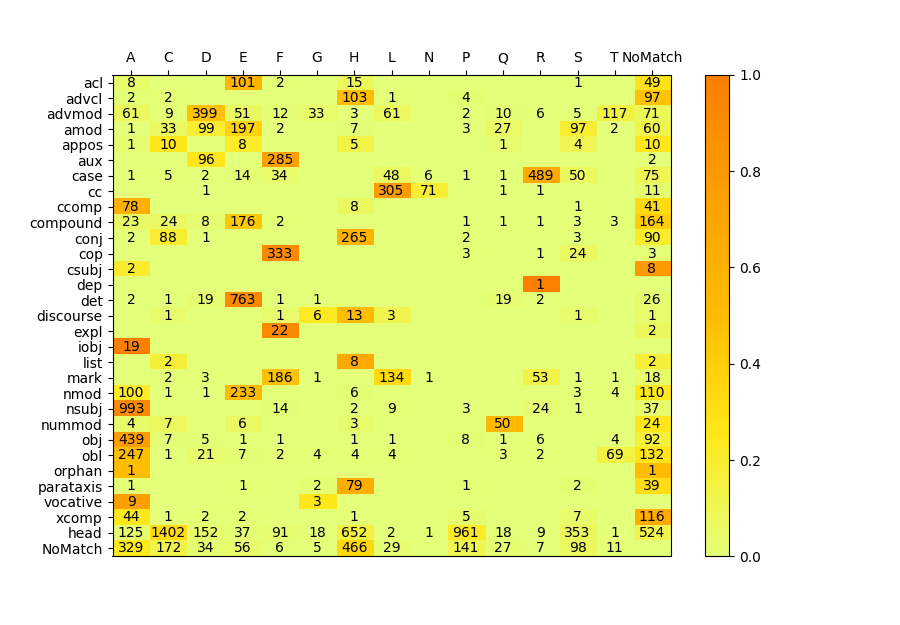
\includegraphics[width=1.15\textwidth]{confusion_matrix.png}
\end{frame}

\begin{frame}
\frametitle{Divergences}
\centering
\begin{tabular}{cc}
\bf UCCA & \bf UD \\\\
Scene/non-Scene & POS-based distinction \\\\
primary/secondary relations, & core/non-core arguments \\
participants & \\\\
more MWEs & less MWEs \\\\
Participant/Elaborator/ & coordination/subordination/ \\
Parallel Scenes & complementation/parataxis
\end{tabular}

\begin{minipage}{.4\textwidth}
  \scalebox{.8}{
    \begin{tikzpicture}[level distance=9mm, sibling distance=14mm, ->, draw=Indigo,
        every circle node/.append style={fill=Indigo}]
      \tikzstyle{word} = [font=\rmfamily,color=black]
      \node (ROOT) [circle] {}
        child {node (After) [word] {After} edge from parent node[above] {\scriptsize $L$}}
        child {node (graduation) [circle] {}
        {
          child {node [word] {graduation} edge from parent node[left] {\scriptsize $P$}}
        } edge from parent node[right] {\scriptsize $H$} }
        child {node [word] {,} edge from parent node[below] {\scriptsize $U$}}
        child {node (moved) [circle] {}
        {
          child {node (John) [word] {John} edge from parent node[left] {\scriptsize $A$}}
          child {node [word] {moved} edge from parent node[left] {\scriptsize $P$}}
          child {node [circle] {}
          {
            child {node [word] {to} edge from parent node[left] {\scriptsize $R$}}
            child {node [word] {Copenhagen} edge from parent node[right] {\scriptsize $C$}}
          } edge from parent node[above] {\scriptsize $A$} }
        } edge from parent node[right] {\scriptsize $H$} }
        ;
      \draw[dashed,->] (graduation) to node [above] {\scriptsize $A$} (John);
    \end{tikzpicture}
    }
\end{minipage}
\hfill
\begin{minipage}{.5\textwidth}
    \begin{dependency}[text only label, label style={above,font=\tt\scriptsize, color=DarkBlue}, edge style={color=DarkBlue}, font=\scriptsize\rmfamily]
    \begin{deptext}[column sep=.1em,ampersand replacement=\^]
    After \^ graduation \^ , \^ John \^ moved \^ to \^ Copenhagen \\
    \end{deptext}
        \depedge[edge unit distance=1ex]{2}{1}{case}
        \depedge[edge unit distance=1ex]{2}{3}{punct}
        \depedge[edge unit distance=1ex]{5}{4}{nsubj}
        \depedge[edge unit distance=1ex, edge end x offset=-2pt]{5}{2}{obl}
        \depedge[edge unit distance=1ex]{7}{6}{case}
        \deproot[edge unit distance=1.5ex]{5}{root}
        \depedge[edge unit distance=1.5ex]{5}{7}{obl}
    \end{dependency}
\end{minipage}
\end{frame}

\begin{frame}
\frametitle{Conclusion}
\begin{itemize}
 \item UCCA's semantic distinctions require a graph structure including {\color{blue}non-terminals}, {\color{orange}reentrancy} and {\color{red}discontinuity}.
 \item \parser{} is an accurate transition-based UCCA parser,
 	and the \textbf{first} to support UCCA and any DAG over the text tokens.
 \item Outperforms strong conversion-based baselines.
\item Multitask learning across semantic representations
\item In-depth comparison of UCCA and UD
\end{itemize}
\end{frame}

\begin{frame}[allowframebreaks]
\frametitle{References}
\bibliographystyle{apalike}
\tiny\bibliography{references}
\end{frame}

\end{document}
